\clearpage
\normalsize
\renewcommand{\thefigure}{E\arabic{figure}}
\setcounter{figure}{0}
\section*{Extension 1. Adding a second volatility signal}
The preceding paper studies one economic signal: relative implied volatility in approximately 30-day, 25-delta put pairs. Its conclusion proposes allocating across several signals. This follow-up implements a first version of that extension while retaining the original signal, actual-contract simulator and entry-sizing result.

\subsection*{Persistent realized-versus-implied differences}
The second signal asks whether a name's recent options have repeatedly implied more volatility than subsequently realized. For each name, we average completed 30-day realized volatility minus entry ATM call IV over the preceding year. Only outcomes finished before the decision enter this memory. We rank eligible names daily and sell the bottom decile: the names with the most persistent negative RV-minus-IV history. This simple persistence forecast avoids changing the original pair signal.

We express the signal through approximately 30-day ATM straddles: equal-count short calls and puts with the same underlying, strike, expiry and adjustment. The combined reference vega is \$450 per IV point. Delta is hedged daily and contracts normally run to expiry. The original call-IV input is retained when moving from calls to straddles. The simulator applies the same funded cash-flow accounting, evaluation execution charges, dividends, financing and admission framework as before.

\subsection*{Learning size within the second signal}
A monthly ridge score partitions proposals into three contexts using 60 months of completed history. The inputs include IV, completed RV-minus-IV memory, VIX, recent IV/VIX changes and a causal fixed-half benchmark's trailing performance and capital use. Exhaustive search over 27 maps assigns 50\%, 75\% or 100\% size to each context to maximize daily training Sharpe. All 35,774 proposals remain; early months use half size until enough completed examples exist.

\begin{center}\small\resizebox{\textwidth}{!}{\begin{tabular}{lllll}\toprule
Straddle entry policy & 2018--21 Sharpe & 2022--25 Sharpe & Later entries & Later profit\\\midrule
Fixed 50\% & 0.740 & 0.920 & 1782 & \$1.824m\\
Fixed 75\% & 0.542 & 0.968 & 1222 & \$2.010m\\
Fixed 100\% & 0.528 & 0.990 & 940 & \$2.206m\\
Contextual sizing & 0.775 & 1.041 & 1204 & \$2.379m\\
\bottomrule\end{tabular}}\end{center}
The retained bandit improves the historical point estimate against the three fixed sizes. Straddles also generate substantially more dollar profit and return volatility than the original put-pair strategy. This difference creates an allocation problem: how selectively should the portfolio take the larger short-volatility exposure?

\clearpage
\section*{Extension 2. Interpreting entry-size decisions}
\begin{figure}[H]\centering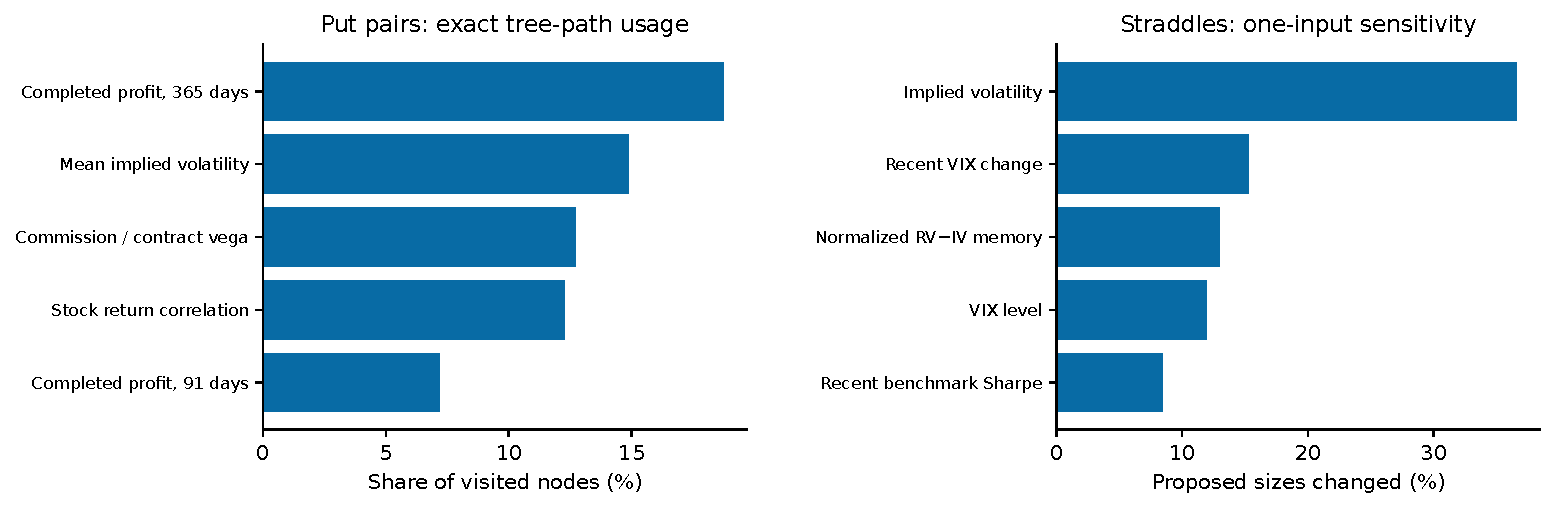
\includegraphics[width=\textwidth]{paper/original_with_rl_extension/figures/bandit_explanations.pdf}\end{figure}
The original put learner can be explained by following its exact tree path and reading the size assigned to the resulting leaf. Completed 365-day profit appears in 18.7\% of later visited decision nodes; mean IV, commission relative to vega and stock-return correlation account for 14.9\%, 12.7\% and 12.3\%. These frequencies describe what the model uses, not whether each feature causes profit.

For straddles, standardized ridge contributions add exactly to a context score; thresholds and the saved context-to-size map then determine exposure. Centering IV changes 36.6\% of fitted later proposal sizes. Recent VIX change changes 15.3\%, normalized RV-minus-IV memory 12.9\% and VIX level 11.9\%. The action map need not be monotonic in the score because it optimizes aggregate Sharpe. All 608 put-pair sizes and 35,774 straddle sizes reproduce the frozen policies exactly.

\begin{center}\small\resizebox{\textwidth}{!}{\begin{tabular}{llll}\toprule
Later entries versus fixed full & Both enter & Bandit only & Fixed only\\\midrule
Original put-pair strategy & 74 & 36 & 1\\
New straddle strategy & 897 & 307 & 43\\
\bottomrule\end{tabular}}\end{center}
The entry benefit combines exposure choices and admission, extending the original paper's capacity diagnostic. Smaller commitments can leave room for later trades. The put bandit admits 110 later entries versus 75 at full size; the straddle bandit admits 1,204 versus 940. These are complete funded policies, rather than size comparisons on identical executed portfolios.

There is also descriptive outcome separation. Among quote-available completed straddle labels, full-size profit averages \$1,631 for later proposals assigned 100\%, versus \$16 for those assigned 50\%. This subset is conditioned on available historical labels. Three within-date size shuffles reach later Sharpes of 0.834, 0.928 and 1.044, versus the bandit's 1.041; one control wins. We therefore separate decision transparency and funded performance from stronger claims of predictive sizing.

\clearpage
\section*{Extension 3. Learning the capital split}
\begin{figure}[H]\centering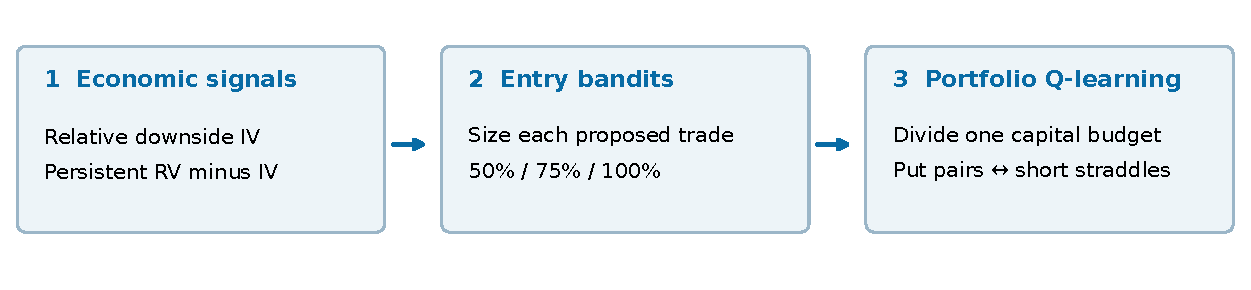
\includegraphics[width=\textwidth]{paper/original_with_rl_extension/figures/learning_layers.pdf}\end{figure}
We freeze the retained put-pair and straddle entry policies and let an outer Q learner allocate one \$10 million budget between their funded strategy indices. Actions choose put/straddle weights of 100/0, 90/10, 75/25, 50/50, 25/75, 10/90 or 0/100. Weights sum to one. All seven fixed benchmarks use the same menu and start at their own split. There is no outer leverage, cash action or additional portfolio stop.

\subsection*{State and execution}
The state combines put-spread strength, the put implied-versus-realized variance-spread feature, straddle IV-versus-RV richness, completed straddle premium, relative strategy volatility, strategy return correlation, VIX, relative recent Sharpe and previous straddle weight. Market information uses the prior close. A weekly decision takes effect at the next close, leaving the first session at old weights. Holdings then drift and affect the cost of the next resize.

The action-value function is quadratic in straddle weight, with coefficients linear in standardized state inputs. Monthly fitted Q iteration uses the preceding 104 completed weeks, requiring 52. The seven prior allocations crossed with seven actions are counterfactuals on the same week; they do not create independent observations. Q uses 50/50 before enough history is available, while fixed controls always use their own target.

\subsection*{Reward and sequential value}
Weekly reward sums daily excess returns normalized by completed training-window reference volatility, then subtracts \(\lambda\) times squared normalized returns. \(\lambda\) controls risk preference. The separate discount \(\gamma\) = 0.99 weights continuation value. Ridge regularization and 200 Bellman updates are held fixed. A matched \(\gamma\) = 0 learner provides a one-period contextual-allocation control.

This is fractional strategy-index allocation, preserving source returns and adding source-based resizing charges. It is not a shared integer-contract replay across both signals. The straddle sleeve introduces net short vega, so the combined portfolio is not vega neutral. The extension tests capital allocation across the existing strategies, while retaining the original contract-level study as its foundation.

\clearpage
\section*{Extension 4. Fixed versus dynamic allocation}
\begin{figure}[H]\centering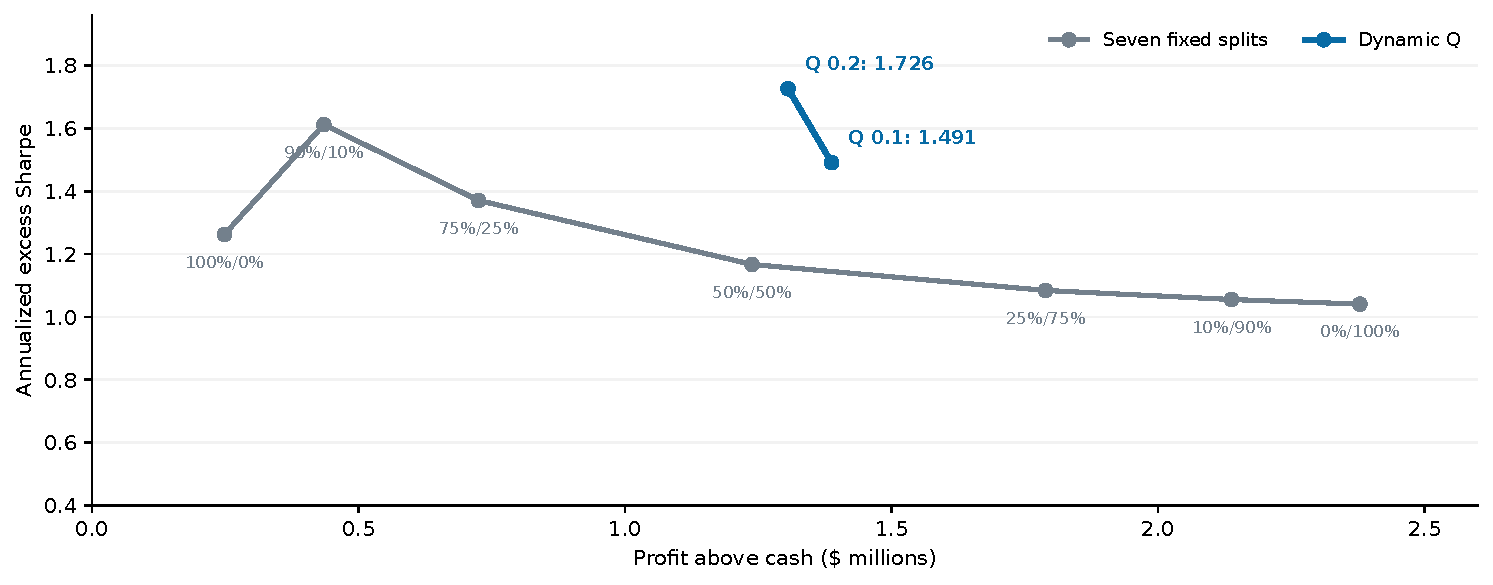
\includegraphics[width=\textwidth]{paper/original_with_rl_extension/figures/q_evaluation.pdf}\end{figure}
\begin{center}\small\resizebox{\textwidth}{!}{\begin{tabular}{llll}\toprule
Put / straddle allocation & 2018--21 Sharpe & 2022--25 Sharpe & Later profit\\\midrule
Fixed 100\% / 0\% & 0.573 & 1.263 & \$0.249m\\
Fixed 90\% / 10\% & 0.926 & 1.612 & \$0.435m\\
Fixed 75\% / 25\% & 0.853 & 1.371 & \$0.726m\\
Fixed 50\% / 50\% & 0.804 & 1.167 & \$1.238m\\
Fixed 25\% / 75\% & 0.785 & 1.084 & \$1.789m\\
Fixed 10\% / 90\% & 0.778 & 1.055 & \$2.138m\\
Fixed 0\% / 100\% & 0.775 & 1.041 & \$2.379m\\
Dynamic Q, \(\lambda\) = 0.1 & 1.286 & 1.491 & \$1.388m\\
Dynamic Q, \(\lambda\) = 0.2 & 1.215 & 1.726 & \$1.306m\\
\bottomrule\end{tabular}}\end{center}
At penalty 0.20, Q reaches later Sharpe 1.726 and \$1.306 million profit above cash. The highest fixed-split Sharpe is 1.612 at 90/10, earning \$435,181. Q also exceeds fixed 50/50 on both Sharpe and profit. Penalty 0.10 trades some Sharpe for profit: 1.491 and \$1.388 million. Straddle-heavy fixed mixes earn more dollars at lower Sharpe, so the gain is a better tradeoff at these operating points, not dominance on every objective.

The put-only endpoint exactly reproduces the original strategy's daily returns and NAV; the straddle-only endpoint reproduces the second strategy. Both periods were previously researched. The two Q preferences are highlighted historical settings, not the highest-validation-Sharpe selections. The complete sweep remains available in the supporting results.

\clearpage
\section*{Extension 5. Why the switches help}
\begin{center}\small\resizebox{\textwidth}{!}{\begin{tabular}{llll}\toprule
Subsequent straddle performance & Mean/day (bps) & Daily vol. (bps) & Conditional Sharpe\\\midrule
Q chose straddles & 3.05 & 16.18 & 3.00\\
Q chose put pairs & 1.30 & 27.00 & 0.76\\
Q chose a mixed split & -2.33 & 20.00 & -1.85\\
\bottomrule\end{tabular}}\end{center}
The allocator's effective distinction is when straddle carry compensates for its risk. After Q chooses straddles, their average excess return is higher and daily fluctuations lower than on dates when Q chooses put pairs. On the latter dates, the put strategy has conditional Sharpe 1.78. The allocator can therefore improve Sharpe while forgoing some average straddle profit.

\begin{figure}[H]\centering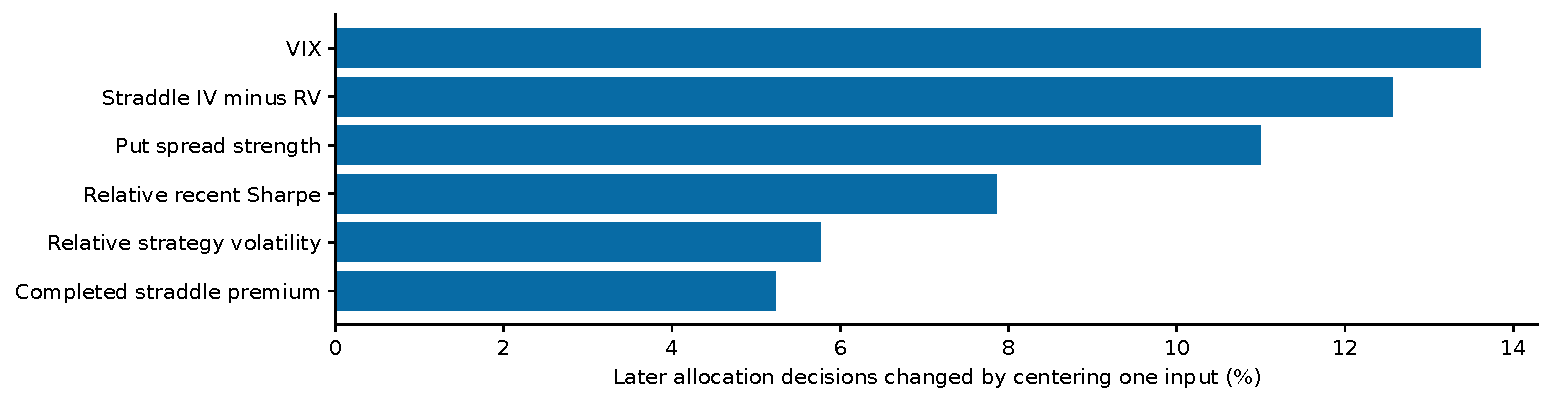
\includegraphics[width=\textwidth]{paper/original_with_rl_extension/figures/q_context.pdf}\end{figure}
\begin{figure}[H]\centering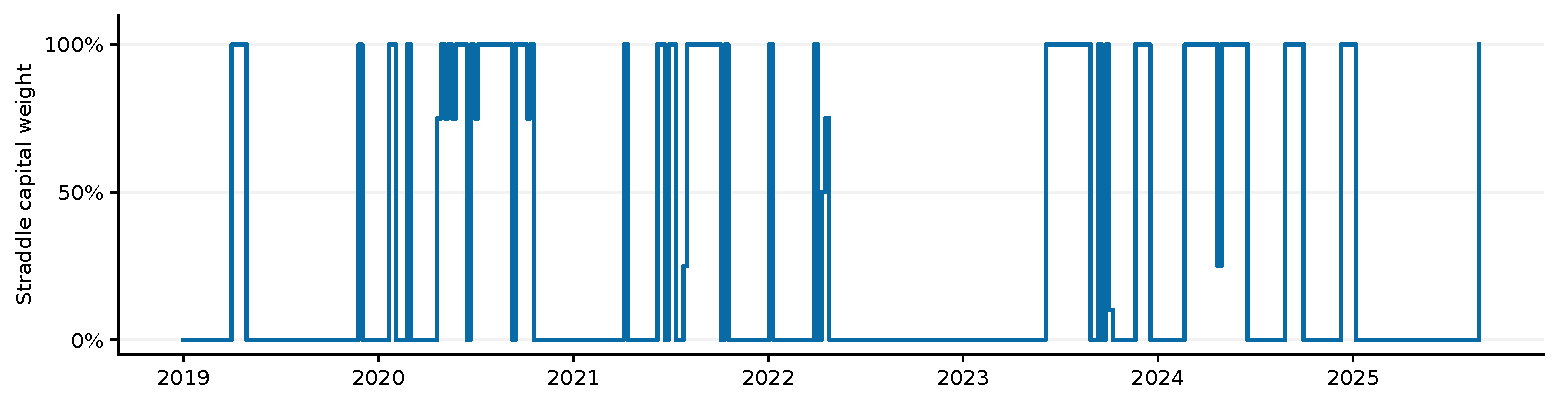
\includegraphics[width=\textwidth]{paper/original_with_rl_extension/figures/q_schedule.pdf}\end{figure}
Of 191 later decisions, 141 choose put pairs alone and 46 straddles alone; only four choose interior splits. Mean straddle target is 24.9\%. In later low-VIX weeks it averages 44.9\%, versus 4.7\% in high-VIX weeks. This median split describes observed behavior, not a fitted threshold rule; the earlier relationship differs. The inputs jointly influence decisions through monthly refits.

The table uses source returns strictly after the decision's execution close through the next execution close. Source costs are included; additional allocation-resizing charges are excluded. These are conditional statistics on noncontiguous historical dates, not separately deployable strategy Sharpes. Centering inputs is a policy sensitivity check, not a causal feature test.

\clearpage
\section*{Extension 6. Timing, continuation and interpretation}
\begin{figure}[H]\centering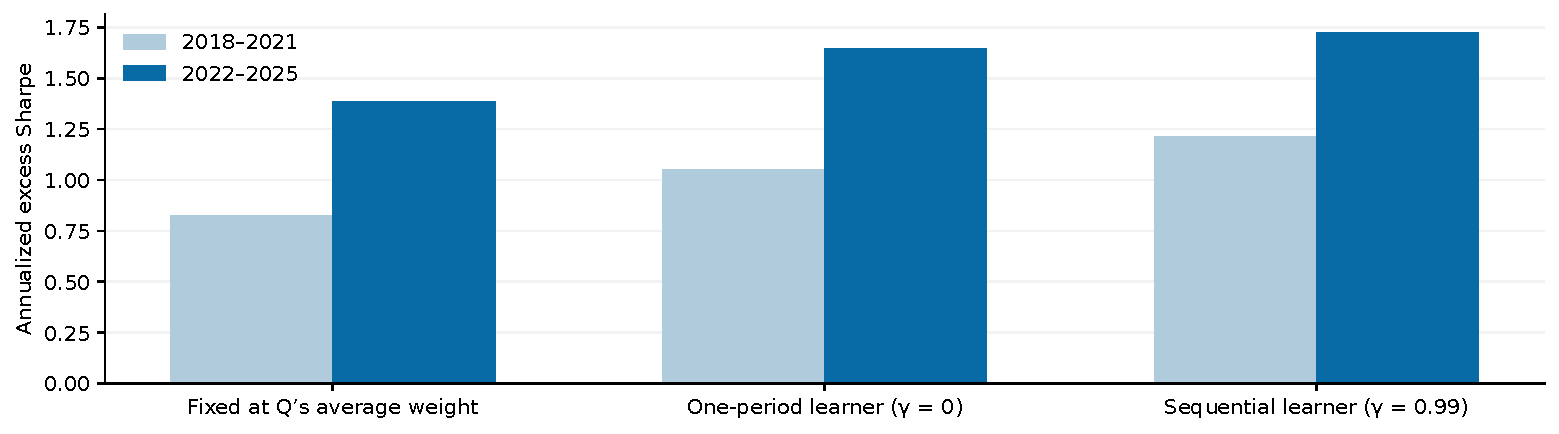
\includegraphics[width=\textwidth]{paper/original_with_rl_extension/figures/q_timing.pdf}\end{figure}
\begin{center}\small\resizebox{\textwidth}{!}{\begin{tabular}{llll}\toprule
Penalty-0.20 policy or control & 2018--21 Sharpe & 2022--25 Sharpe & Later profit\\\midrule
Fixed at Q's mean target & 0.828 & 1.387 & \$0.841m\\
One-period learner, \(\gamma\) = 0 & 1.053 & 1.645 & \$1.184m\\
Sequential Q, \(\gamma\) = 0.99 & 1.215 & 1.726 & \$1.306m\\
\bottomrule\end{tabular}}\end{center}
A constant target equal to Q's later mean straddle allocation gives Sharpe 1.387 and \$841,251 profit, versus Q's 1.726 and \$1.306 million. The earlier comparison is 0.828 versus 1.215. Average exposure alone therefore does not explain the point estimate. These targets use the realized mean retrospectively and are diagnostic rather than validation-selected policies.

Shifting the learned action schedule through 49 nonzero circular offsets, preserving its action counts and most serial structure, gives median later Sharpe 0.744; none reaches Q. Three of 49 earlier rotations reach or exceed the actual policy. Wealth and resizing costs are recomputed. This is descriptive evidence for timing conditional on the researched schedule, not a selection-adjusted significance result.

The matched one-period learner already reaches later Sharpe 1.645. Q's continuation term changes 9 of 191 later decisions when evaluated at the same actual states; it adds a smaller increment than the full dynamic-versus-fixed gap. Some feature-centering interventions also improve Sharpe slightly. The clearest interpretation is conditional allocation with a modest incremental sequential benefit, rather than proof that every input or long-horizon planning is essential.

This extension builds on the original finding rather than replacing it: learn entry size within a signal, then study allocation across distinct signals. Its historical limitations remain. The straddle procedure searched both periods, and the highest-validation-Sharpe Q preference performs poorly later (0.282). Execution assumptions and a shared contract-level allocator still need validation. Supporting controls, complete sweeps and exact explanation files are retained in reports/allocation\_interpretability\_099 and reports/signal\_allocation\_discount.

